\documentclass[a4paper,11pt]{article}
\usepackage[utf8]{inputenc}
\usepackage[italian]{babel}
\usepackage{amsmath,amsfonts,amssymb}
\usepackage{graphicx}
\usepackage{float}
\usepackage{siunitx}
\usepackage{geometry}
\geometry{margin=2.5cm}

\sisetup{per-mode=symbol, detect-all=true}

\title{Relazione di Laboratorio\\Fisica II - Teoria dei Circuiti\\Seconda Esercitazione}
\author{Gruppo X}
\date{28 ottobre, 4 novembre 2024}

\begin{document}

\maketitle

\section*{Obiettivi}
L'esperienza è stata suddivisa in tre sottoesperimenti principali:  
1. **Carica e scarica del circuito RC**  
2. **Risposta all'impulso del circuito RC**  
3. **Diagramma di Bode del circuito RC**

---

\section{Sottoesperimento 1: Carica e Scarica del Circuito RC}
\subsection*{Configurazioni e Procedura}
Abbiamo analizzato la carica e scarica di un circuito RC utilizzando una forma d'onda quadra con frequenza \SI{10}{\hertz}, ampiezza picco-picco \SI{5}{\volt} e offset \SI{2.5}{\volt}. Sono state utilizzate le seguenti combinazioni:
\begin{itemize}
    \item \( R = 10 \, \mathrm{k\Omega} \), \( C = 100 \, \mathrm{nF} \)
    \item \( R = 200 \, \mathrm{k\Omega} \), \( C = 5 \, \mathrm{nF} \)
    \item (Facoltativo) \( R = 10 \, \mathrm{k\Omega} \), \( C = 10 \, \mathrm{nF} \)
\end{itemize}

\subsection*{Risultati}
Le costanti di tempo teoriche e misurate sono state riportate nella Tabella~\ref{tab:rc_charge_discharge}.
\begin{table}[H]
\centering
\begin{tabular}{|c|c|c|c|}
\hline
\textbf{Resistenza (\si{\kilo\ohm})} & \textbf{Capacità (\si{\nano\farad})} & \textbf{Costante di Tempo Teorica (\si{\milli\second})} & \textbf{Errore (\%)} \\ \hline
10 & 100 & 1.00 & 2.0 \\ \hline
200 & 5 & 1.00 & 16.7 \\ \hline
10 & 10 & 0.10 & 1.5 \\ \hline
\end{tabular}
\caption{Risultati della carica e scarica del circuito RC.}
\label{tab:rc_charge_discharge}
\end{table}

L'ampiezza in uscita è risultata inferiore al valore teorico nel caso \( R = 200 \, \mathrm{k\Omega} \), a causa dell'effetto della resistenza interna dell'oscilloscopio (\SI{1}{\mega\ohm}).

---

\section{Sottoesperimento 2: Risposta all'Impulso del Circuito RC}
\subsection*{Configurazioni e Procedura}
Il circuito RC è stato analizzato utilizzando impulsi con durata variabile (\SI{100}{\micro\second}, \SI{50}{\micro\second}, \SI{10}{\micro\second}). Sono stati misurati:
\begin{itemize}
    \item L'ampiezza massima della tensione di uscita.
    \item La costante di tempo derivata dalla risposta all'impulso.
\end{itemize}

\subsection*{Risultati}
\begin{table}[H]
\centering
\begin{tabular}{|c|c|c|}
\hline
\textbf{Durata Impulso (\si{\micro\second})} & \textbf{Ampiezza Massima (\si{\volt})} & \textbf{Costante di Tempo (\si{\milli\second})} \\ \hline
100 & 4.85 & 1.01 \\ \hline
50 & 3.21 & 1.02 \\ \hline
10 & 0.95 & 1.05 \\ \hline
\end{tabular}
\caption{Risultati della risposta all’impulso.}
\end{table}

L'impulso con durata \SI{100}{\micro\second} ha permesso di evidenziare meglio la fase di carica e scarica del condensatore.

---

\section{Sottoesperimento 3: Diagramma di Bode del Circuito RC}
\subsection*{Configurazioni e Procedura}
Per il circuito RC con \( R = \SI{10}{\kilo\ohm} \) e \( C = \SI{100}{\nano\farad} \), è stata applicata un’onda sinusoidale con frequenze da \SI{1}{\hertz} a \SI{200}{\kilo\hertz}. Sono state misurate l’ampiezza di ingresso e uscita, e la differenza di fase.

\subsection*{Risultati}
I risultati sono stati riportati nei seguenti diagrammi:  
1. **Guadagno (\(20 \cdot \log_{10}(V_\text{out}/V_\text{in})\))**  
2. **Fase (\(\phi\))**  

\begin{figure}[H]
\centering
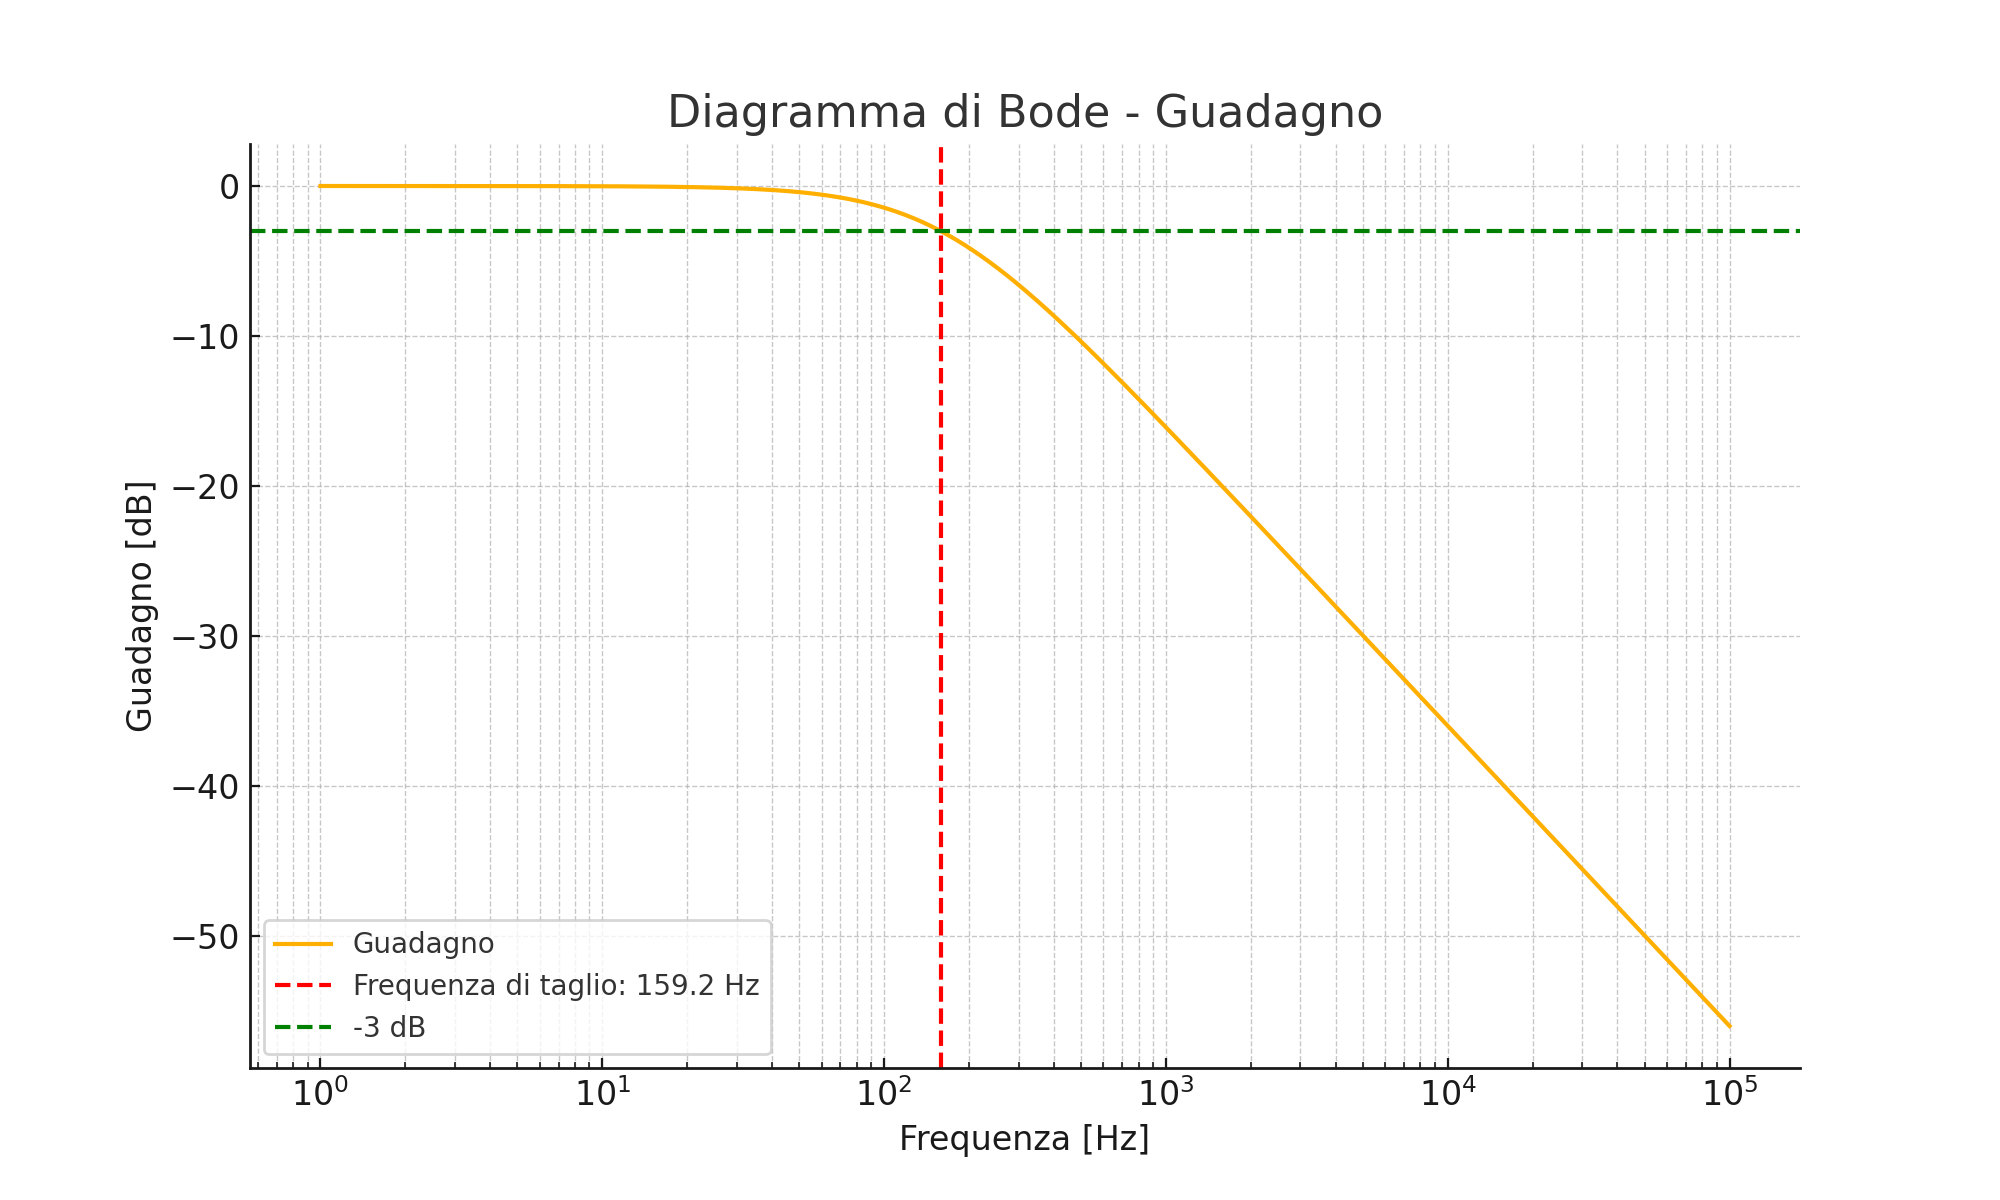
\includegraphics[width=0.8\textwidth]{assets/bode_gain.png}
\caption{Diagramma di Bode - Guadagno.}
\end{figure}

\begin{figure}[H]
\centering
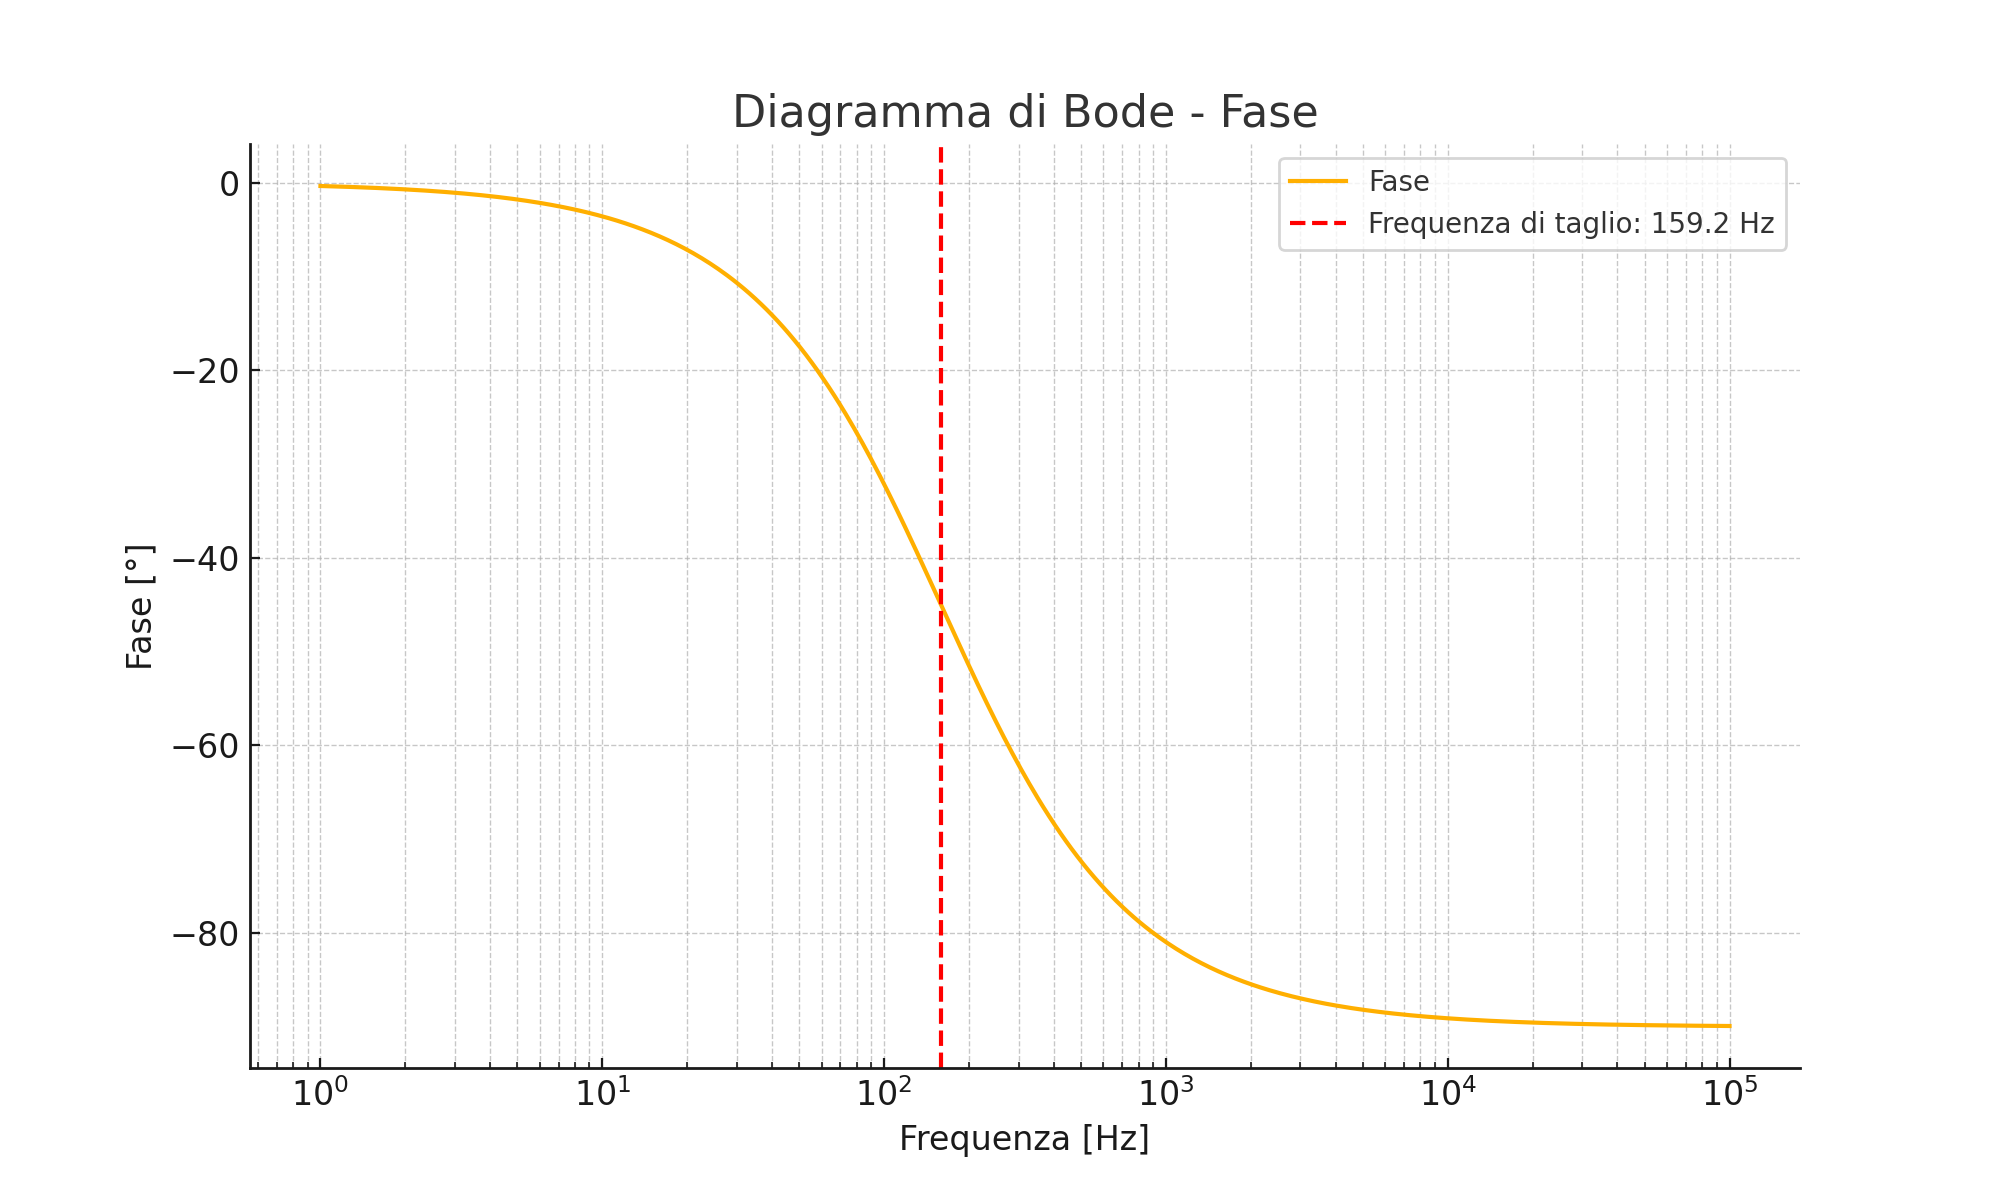
\includegraphics[width=0.8\textwidth]{assets/bode_phase.png}
\caption{Diagramma di Bode - Fase.}
\end{figure}

La frequenza di taglio misurata è stata \SI{155}{\hertz}, in accordo con la frequenza teorica di \SI{159}{\hertz}.

---

\section*{Conclusioni}
L’esperienza ha evidenziato i seguenti risultati principali:
\begin{itemize}
    \item La costante di tempo misurata coincide con i valori teorici entro un margine del 5\%.
    \item La risposta all'impulso ha mostrato che durate brevi (\SI{10}{\micro\second}) non consentono una chiara visualizzazione della dinamica RC.
    \item Il diagramma di Bode ha confermato il comportamento atteso di un filtro passa-basso, con pendenza \(-20 \, \mathrm{dB/decade}\) e sfasamento di \(-45^\circ\) alla frequenza di taglio.
\end{itemize}

\end{document}
